%% -*- LaTeX -*-
\documentclass{report}

\usepackage{thesis}

%some other packages I found useful, comment out or remove if you do not need them
\usepackage{amsmath}
\usepackage{amssymb}
\usepackage[titletoc,toc,title]{appendix}
\usepackage{chapterbib}
\usepackage{cite}
\usepackage[pdftex]{graphicx}
\usepackage{mdframed}
\usepackage{minted}
\usepackage{multirow}
\usepackage{pdfcomment}
\usepackage{subfigure}
\usepackage{tabularx}
\usepackage{titlesec}
\usepackage{url}
\usepackage{xspace}

% must be loaded after hyperref
\usepackage{cleveref}

\newcommand{\inlinecode}[2][haskell]{\mintinline[breaklines]{#1}{#2}}

\newcommand{\ChoreographyTS}{ChoreoTS\xspace}
\newcommand{\chorLambda}{Chor$\lambda$\xspace}
\newcommand{\Chorus}{ChoRus\xspace}
\newcommand{\HasChor}{Has\-Chor\xspace}
\newcommand{\HLSCentral}{$\boldsymbol{\lambda}_{\boldsymbol{C}}$\xspace}
\newcommand{\HLSLocal}{$\boldsymbol{\lambda}_{\boldsymbol{L}}$\xspace}
\newcommand{\HLSNet}{$\boldsymbol{\lambda}_{\boldsymbol{N}}$\xspace}
\newcommand{\MultiChor}{Multi\-Chor\xspace}

\widowpenalty=1000000
\clubpenalty=1000000


\title{Choreographic Programming 2: Electric Boogalo}
\author{Mako Bates}
\defensedate{June XX, 2025}
\dissertation                             %% or \dissertation
\doctorphilosophy                      %% or \doctorphilosophy or \masterarts
\cs                                 %% this is the only speciality defined.
\graduatingIn{August}
\advisor{Bunny Lebowski, Ph.D.}
\readerone{Walter Sobchak, Ph.D.}
\readertwo{Carl Hungus, Ph.D.}      %% Optional if MS.
\chair{V.I. Lenin, Ph.D.}
\dean{Holger Hoock, Ph.D.}  %% TODO: check title.


\begin{document}
\maketitle
\makeacceptance

\begin{abstract}
Presents both MultiChor (and possibly a distinct variant MiniChor) and a formalism "He Lambda something".
Shows how this system is more ergonomic than prior work and equally as expressive.
Expolores the theoretical minimum of choreographic programming, and implications for real use.
\end{abstract}

\begin{citationspage}
\citationheadingpublished
\noindent Doe, J. and B. Lebowski. (2009). My First Published Paper. {\it Proceedings of the IEEE Congress on Life}.
\\ \\
\noindent Doe, J. and B. Lebowski. (2010). My Second Published Paper. {\it The World's Greatest Journal}.

%if have unpublished work, use one or more of the following
\begin{center}
\vskip 2em
{\large AND}
\end{center}
\vskip 2em 
Material from this dissertation has been accepted for publication in {\it Fantastic Journal} on 05/20/2013 in the following form:\\
\vskip 2em 
\noindent Doe, J. and B. Lebowski. (2013). Soon To Be Published Paper. {\it Fantastic Journal}.

\begin{center}
\vskip 2em
{\large AND}
\end{center}
\vskip 2em 
Material from this dissertation has been submitted for publication in {\it Some Other Journal} on 04/30/2013 in the following form:\\
\vskip 2em 
\noindent Doe, J. and B. Lebowski. (2013). Paper In Review. {\it Some Other Journal}.

\end{citationspage}

\begin{dedication} %% Optional
{\large 
{\it in memory of} 
\\
\vskip 2em
Alan Turing (1912-1954)}
\end{dedication}

\begin{acknowledgements}  %% Optional
I'd like to take this opportunity to pour a little of my 40oz. out for all
the homies that didn't make it.
\end{acknowledgements}

\tableofcontents
\listoffigures
\listoftables

\mainmatter
\sloppy

%for journal format dissertation each chapter needs its own reference section, and want references to be included in global bibliography
%this is accomplished using include commands
%but, for things like the lit review (chapter 1) or an appendix, should use input so it does not get it's own references section

%if not doing a journal format dissertation you can just use input for all chapters, or put text here directly.
\chapter{Introduction and Literature Review}

\begin{quote}
Chapter abstract goes here.
I should check if the concept of "Introduction \emph{and} Lit Review" is required.
Having an abstract for the introduction seems dumb, and I'm not sure I want a monolithic lit review up front.
\end{quote}

\section{Introduction}

We're talking about Choreographic Programming (CP).

\section{An illustrative example}

\Cref{fig:kvsenclave} shows an example choreography.
Probably a KVS variation.
Here we describe what it does and how to read it.

\begin{figure}[tbhp]\caption{Example Choreography: a key-value store}
  \begin{mdframed}
  \begin{tabular}{c c}
  \begin{minipage}{8.75cm}
    \inputminted[xleftmargin=10pt,linenos,fontsize=\scriptsize]{haskell}{figures/kvsenclave_a.hs.txt}
  \end{minipage}
  &
  \begin{minipage}{3.75cm}
    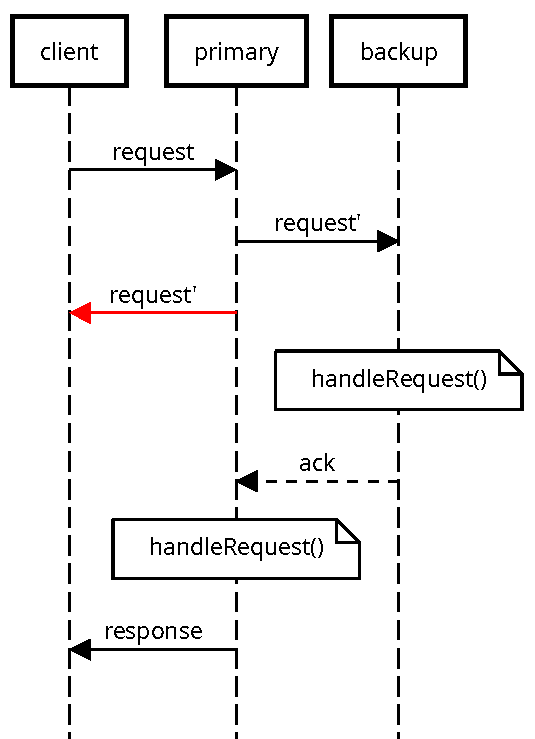
\includegraphics[width=4cm]{figures/seq2.pdf}
  \end{minipage} \\\\
  \multicolumn{2}{c}{\begin{minipage}{12.5cm}
  A key-value store with a backup server, written in \MultiChor.
           The backup server sends an acknowledgement message \textsf{ack} to the primary server
           if and only if \inlinecode{request} is a \inlinecode{Put}.
           The \inlinecode{broadcast} operator (line 19) ensures KoC
           so that the primary and backup servers are guaranteed to use the same case of \inlinecode{handleBackup},
           but it results in redundant communication (shown in red in the sequence diagram).
  \end{minipage}}\\\\
  \hline\\
  \begin{minipage}{8.75cm}
    \inputminted[xleftmargin=10pt,linenos,fontsize=\scriptsize]{haskell}{figures/kvsenclave_b.hs.txt}
  \end{minipage}
  &
  \begin{minipage}{3.75cm}
     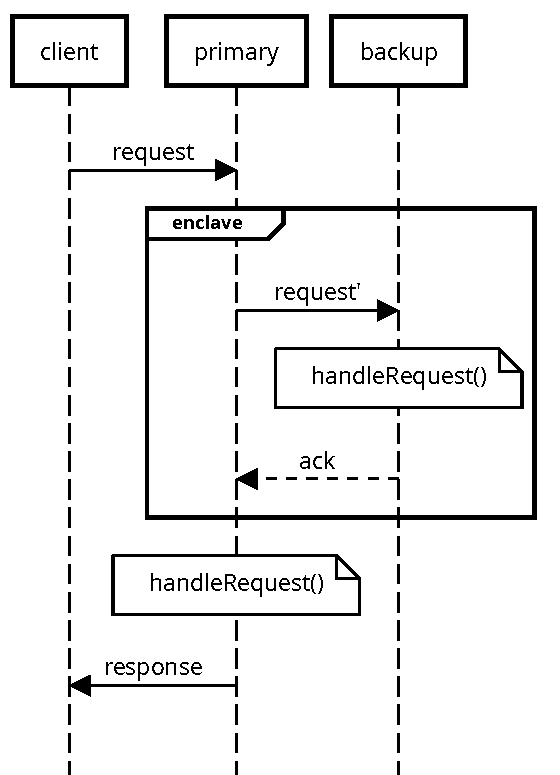
\includegraphics[width=4cm]{figures/seq3.pdf}
  \end{minipage} \\\\
  \multicolumn{2}{c}{\begin{minipage}{12.5cm}
  In this variation, the \inlinecode{enclave} operator eliminates the redundant communication.
           The enclaved sub-choreography is indicated by a box in the sequence diagram.
           On line~2, \inlinecode{@@ nobody} is \MultiChor idiom explained in \Cref{sec:membership}.
  \end{minipage}}
  \end{tabular}
  \label{fig:kvsenclave}
    %%\Description{In the top section, twenty four lines of Haskell code using the MultiChor library, with a UML sequence diagram of that program.
%%	The code defines a choreography called "kvs", and helper-functions "handleRequest" and "handleBackup".
%%	In the sequence diagram, first "client" sends "request" to "server",
%%	  then "server" sends "request-prime" to "client" and "backup",
%%	  then backup calls "handleRequest",
%%	  then backup may send "ack" to "server",
%%	  then server calls "handleRequest",
%%	  then server sends "response" to "client.
%%	The bottom sections shows changes to the code in the top section.
%%	In particular, the return type of "handleBackup" is changed to exclude "client".
%%	In the updated sequence diagram, the part of the protocol representing "handleBackup" is in a box named "enclave",
%%	  and the spurious transmission of "request-prime" from "server" to "client" is omitted.
%%	  }
  \end{mdframed}
\end{figure}


Here is a citation, \shortcite{skalka-smith-aplas04}.

\section{Layout and Contributions}

The remainder of this chapter covers the history and theory of CP
and discusses some modern work relevant to the ongoing development of CP systems.
In particular, \Cref{sec:koc-strategies} discusses the "Knowledge of Choice" problem,
a central difficulty in the design of CP systems,
and a number of strategies that have been used to solve it.

\Cref{sec:asdf} should be highlited?	


\chapter{My First Published Paper}
\chaptermark{First Paper} %this is the chapter heading that will show on subsequent pages
\label{sec:asdf}

\begin{quote}
Paper abstract
\end{quote}


\section{Introduction}
Here is a citation \shortcite{Bongard2009}.

\bibliographystyle{chicago}
\bibliography{example}

\chapter{My Second Published Paper}
\chaptermark{Second Paper} %this is the chapter heading that will show on subsequent pages

\begin{quote}
Paper abstract
\end{quote}


\section{Introduction}
Here is a different citation \shortcite{Bongard2000}.  

\subsection{More Details}

And one more \shortcite{AuerbachBongard2010}.

\bibliographystyle{chicago}
\bibliography{example}


\bibliographystyle{chicago}
\bibliography{example}

\appendix
\addappheadtotoc

\titleformat{\chapter}[hang] 
{\normalfont\huge\bfseries}{\chaptertitlename\ \thechapter:}{1em}{} 

\chapter{Parameters}
\label{journal:app:Params}
\begin{table}[h!]
\caption{Algorithm Parameters.}
\begin{center}
\begin{tabularx}{\textwidth}{ |X|X| }
%\begin{tabular}{|l|l|}
\hline
 {\bf Parameter Name} & {\bf Value}  \\ \hline \hline
 %\multicolumn{2}{|c|}{Evolutionary Algorithm Parameters} \\
 %\hline
 Population Size & 1000 \\
 Max Generations & 5000 \\ 
 Mutation Rate  & 0.03 \\
 \hline
\end{tabularx}
\end{center}
\vspace{-0.4cm}
\label{journal:tab:Params1}
\end{table} 



\end{document}
